\documentclass{article}
\author{Lena Morrill}
\date{\today}
\title{Addressing Thomas' comments}

\usepackage{tikz}
\usepackage{lscape}
\usepackage{array}
\usepackage{graphicx}
\usepackage{hyperref}
\usepackage{dsfont}

\setlength{\textwidth}{6.7in}
\setlength{\oddsidemargin}{-0.1in}
\setlength{\textheight}{8.6in}
\setlength{\topmargin}{-0.4in}

\def\checkmark{\tikz\fill[scale=0.4](0,.35) -- (.25,0) -- (1,.7) -- (.25,.15) -- cycle;} 
\newcolumntype{L}[1]{>{\raggedright\let\newline\\\arraybackslash\hspace{0pt}}m{#1}}
\newcolumntype{C}[1]{>{\centering\let\newline\\\arraybackslash\hspace{0pt}}m{#1}}
\newcolumntype{R}[1]{>{\raggedleft\let\newline\\\arraybackslash\hspace{0pt}}m{#1}}


\begin{document}
\maketitle

\tableofcontents

\section{scDNA}

Thomas made the comment that it would be useful to have a metric of heterogeneity within an organoid, computed using the scDNA data.

\begin{figure}[h]
\includegraphics[width=\textwidth]{/Users/morril01/Documents/PhD/other_repos/Vias_Brenton/scDNAseq-Organoids/plots/subclonal_hclust_CI_across_genome_2.pdf}
\caption{90\% confidence intervals for the centered copy number (centered around the mean of each bin), for all 3 organoids for which we have scDNA. Loci with a larger shaded area indicate loci of higher variance in CN across cells, suggesting subclonal heterogeneity. The colour of the dots (difficult to see, but they are the lines along the $x$ axis at $y=0$) is a gross approximation of the clonal (blue) or subclonal (red) status of each bin in each sample, with blue colours indicating loci with no variability in copy number. }
\end{figure}

However, an important realisation when analysing these data is that the variance and the mean copy number for each bin have a correlation (i.e. the data are heteroscedastic). You can see this relationship in the plot below.

\clearpage

\begin{figure}[h]
\centering
\includegraphics[width=.6\textwidth]{/Users/morril01/Documents/PhD/other_repos/Vias_Brenton/scDNAseq-Organoids/plots/subclonal_hclust_CI_across_genome_heteroscedasticity.pdf}
\caption{Mean/ standard deviation relationship in binned copy number values}
\end{figure}

\textbf{Note: what follows I have to check with Dom} I fit a linear model \verb|Sd~Mean| and find the expected variance $\mathds{E}(\sigma^2)$. I then compare $\mathds{E}(\sigma^2)$ to the observed variance $S^2$ in each bin in each sample with a Chi-Squared test,~\footnote{\url{https://www.rdocumentation.org/packages/EnvStats/versions/2.3.1/topics/varTest}} in which my alternative hypothesis is that $\mathds{E}(\sigma^2) < S^2$ . A statistically significant result indicates that we see a greater variance than expected in the copy number values of this bin, and that therefore there is subclonal heterogeneity. The fraction of statistically significant bins can be found in the table below, indicating that PDO3 is the most heterogeneous sample (i.e. the one that presents highest levels of subclonal heterogeneity), followed by PDO2 and PDO6, which present similar levels.

% latex table generated in R 4.0.3 by xtable 1.8-4 package
% Wed Jun 23 11:53:26 2021
\begin{table}[ht]
\centering
\begin{tabular}{rr}
  \hline
 & fraction\_heterogeneous \\ 
  \hline
PDO3 & 0.48 \\ 
  PDO6 & 0.26 \\ 
  PDO2 & 0.29 \\ 
   \hline
\end{tabular}
\end{table}


\section{Transcriptomics}
\subsection{Use of DESeq $vs$ TPM, and of absolute CN $vs$ relative CN}
Several of Thomas' comments were that he thought we should use TPM instead of DESeq2 counts, and relative CN instead of absolute CN, for the gene expression $vs$ copy number correlation analysis of Fig3.

\begin{itemize}
\item My thoughts on using relative CN: if using TPM, the use of relative (as opposed to absolute) CN would only be useful to retrieve the true CN-GE correlations if there was a perfect scaling of CN and GE in all genes. If not, the data gets deformed due to the normalisation both for CN and for GE, but independently (which doesn't help us find the true correlations). We know that GE and CN don't scale, but that instead the changes in CN sometimes lead to changes in GE, sometimes not. Overall, I don't see the benefit of using relative CN in this context
\item His reasoning to use TPM instead of DESeq2 counts is that we can have some outlier samples (e.g. MYC-amplified) for which the gene expression values are very different from the values of the rest of the samples. Given that DESeq2 normalises the genes both within a sample and between samples (using a geometric mean) he thought it would be a bad idea to use a normalisation that uses all samples. (TPM doesn't; it only takes into account counts from the sample and normalises it to a total of a million transcripts). I was hoping that because the DESeq2 normalisation is very robust, using DESeq2 counts would give more robust results than using alternatives, including TPM. 
\item Some downsides (from my point of view) of using TPM is that we still see a deformation of the data due to phenomena such as MYC amplification (e.g. if MYC amplification leads to general up-regulation of many genes in its pathway, then the TPM of the remaining genes will decrease due to the normalisation). Thomas was not convinced by this argument and I wasn't too sure either; I think we rather reached the conclusion that both types of normalisation have their downsides
\end{itemize}

I am still in the process of re-creating the plots in Fig3 using TPM instead of DESeq2 counts. A preliminary result is that the plot in fig3c shows practically the same ranking of the genes of interest when using TPM instead of DESeq2. There is a good correlation between TPM counts and DESeq2 anyway; I don't expect results to change too much.

\subsection{How to understand the PCA}
One of his criticisms was that we didn't explain the PCA of RNA-Seq samples, and it is true that we have tried a lot to understand what is going on at the transcriptomic level without much success.

The old PCA, using 15 samples, which is the one included in the paper, was created using DESeq2 counts (normalised with tumour and normal fallopian tube samples), and is

\begin{figure}[h]
\centering
\includegraphics[width=3in]{/Users/morril01/Documents/PhD/other_repos/Vias_Brenton/RNASeq_DE_resistant_sensitive/figures/PCA_RNASeq_with_more_samples/PCA_counts_subset_BRCA_TAMSeq.png}
\end{figure}

i.e. showing PDO4, PDO13 and PDO17 really separated along the first PC. The pair PDO7 and PDO8 are moderately separated, PDO5 and PDO6 appear together, and PDO3 and PDO9 are very similar in PC1, but not in PC2.

In trying to understand why we were getting somewhat strange results for the RNASeq analysis I looked at the absolute TPM counts for all samples that we had included, and saw that in some cases some samples had extremely high values (including normal samples). That made me think again that perhaps we should have been more stringent in removing samples with 3' bias. I had originally removed from the analysis PDO18, PDO16 and PDO14. Stephane had removed a further sample, PDO17, when he did the differential abundance analysis of normal fallopian tube $vs$ organoids. You can see in Figure~\ref{bias} the 3' bias for each organoid sample.
\clearpage

\subsubsection{Re-analysis including on 11 samples}
In the analyses that follow I have removed all samples with any indication of 3' bias (i.e. the ones mentioned above, plus PDO4, PDO13, and PDO9).

\begin{figure}[h]
\centering
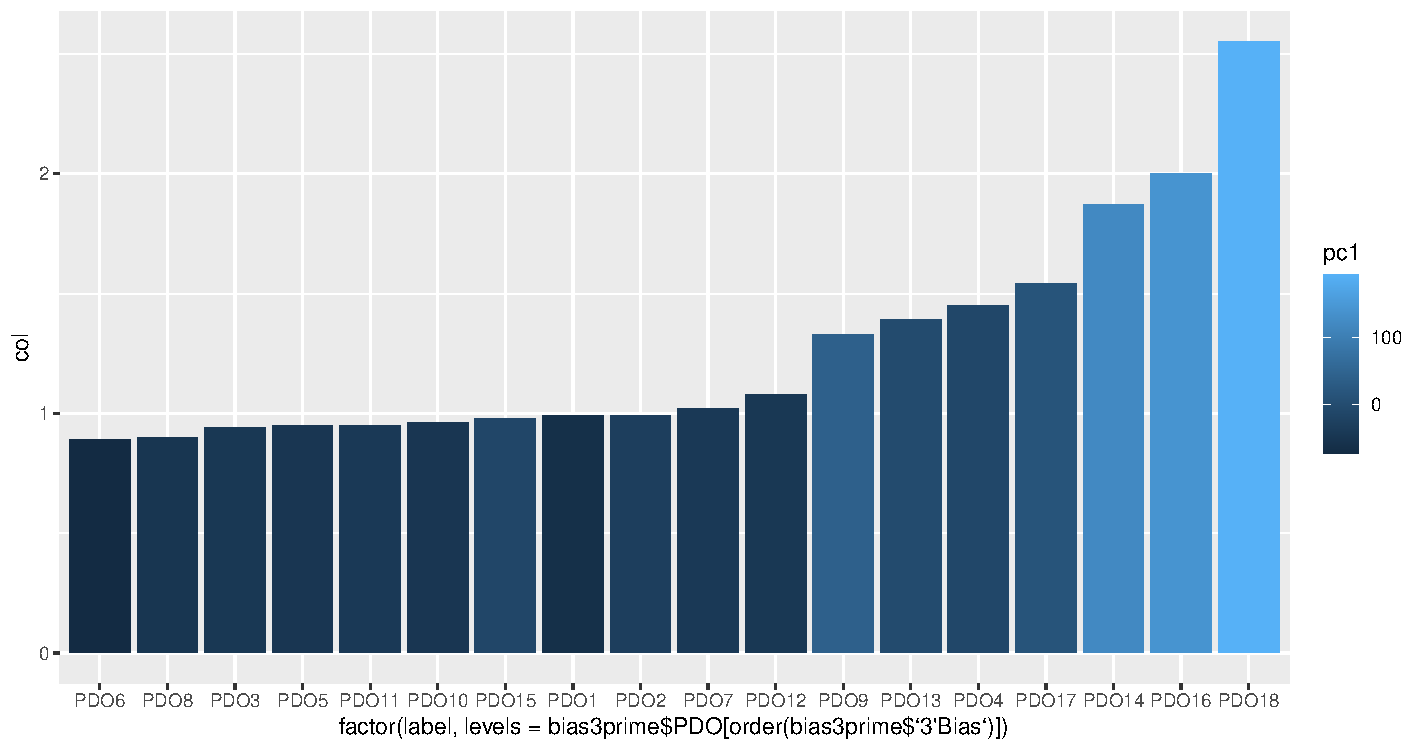
\includegraphics[width=5.2in]{../../RNASeq_DE_resistant_sensitive/figures/PCA_RNASeq_with_more_samples/3primebias_barplot_counts.pdf}
\caption{3' bias for organoid samples\label{bias}}
\end{figure}

I have re-normalised the counts using DESeq2 when only including these 11 samples which should be free of 3' bias. There are some things we could explain better once we only keep 11 samples:
\begin{itemize}
\item PDO3 and PDO9 seemed to be quite different in their transcriptomics even though they come from the same patient. I had tried to see what were the differences between the two and couldn't find anything. If we remove PDO9 due to 3' bias, this could explain why the two samples are different and it's difficult to find any biological interpretation for such a difference - it's a technical artefact
\item The first PC, which shows PDO4, PDO13 and PDO17 on the left side of the PCA plot, show the same artefactual difference. The fact that I could not annotate genes that explain the variance in the first PC would also be explained.
\end{itemize}


\begin{figure}[h]
\centering
\includegraphics[width=3.2in]{../../RNASeq_DE_resistant_sensitive/figures/PCA_RNASeq/PCA_counts_subset_BRCA_TAMSeq.png}
\includegraphics[width=3.2in]{/Users/morril01/Documents/PhD/other_repos/Vias_Brenton/RNASeq_DE_resistant_sensitive/figures/other_DE/pathways_heatmap_orgs.pdf}
\caption{PCA with only 11 samples, and enrichment of pathways of interest\label{newpca}}
\end{figure}

The new PCA, created with DESeq2 counts from this subset of 11 samples, is shown in Figure~\ref{newpca}. We see how the second principal component of the PCA with 15 samples is now the first PC of the PCA with 11 samples. 
\begin{itemize}
\item PDO5 and PDO6 are shown to be different from the rest of the samples in this first PC, but very similar to each other. 
\item PDO7 and PDO8 still are a bit separated.
\item PDO2 and PDO10 appear to be very similar. When doing onthology /enrichment analysis using REACTOME pathways, we see that both are active in the homologous recombination pathway. These are the only two organoids with very high exposure of s7. I think this is a pontentially nice result!
\item PDO5 and PDO6 have a slight high enrichment in the ERBB pathway
\item I was creating the results from fig 3 with only this subset of 11 samples but I haven't had time to finish it
\item The annotation of the loadings in this new PCA might be easier to understand than in the previous version of the PCA (see Figure~\ref{anno})
\end{itemize}

\begin{figure}[h]
\centering
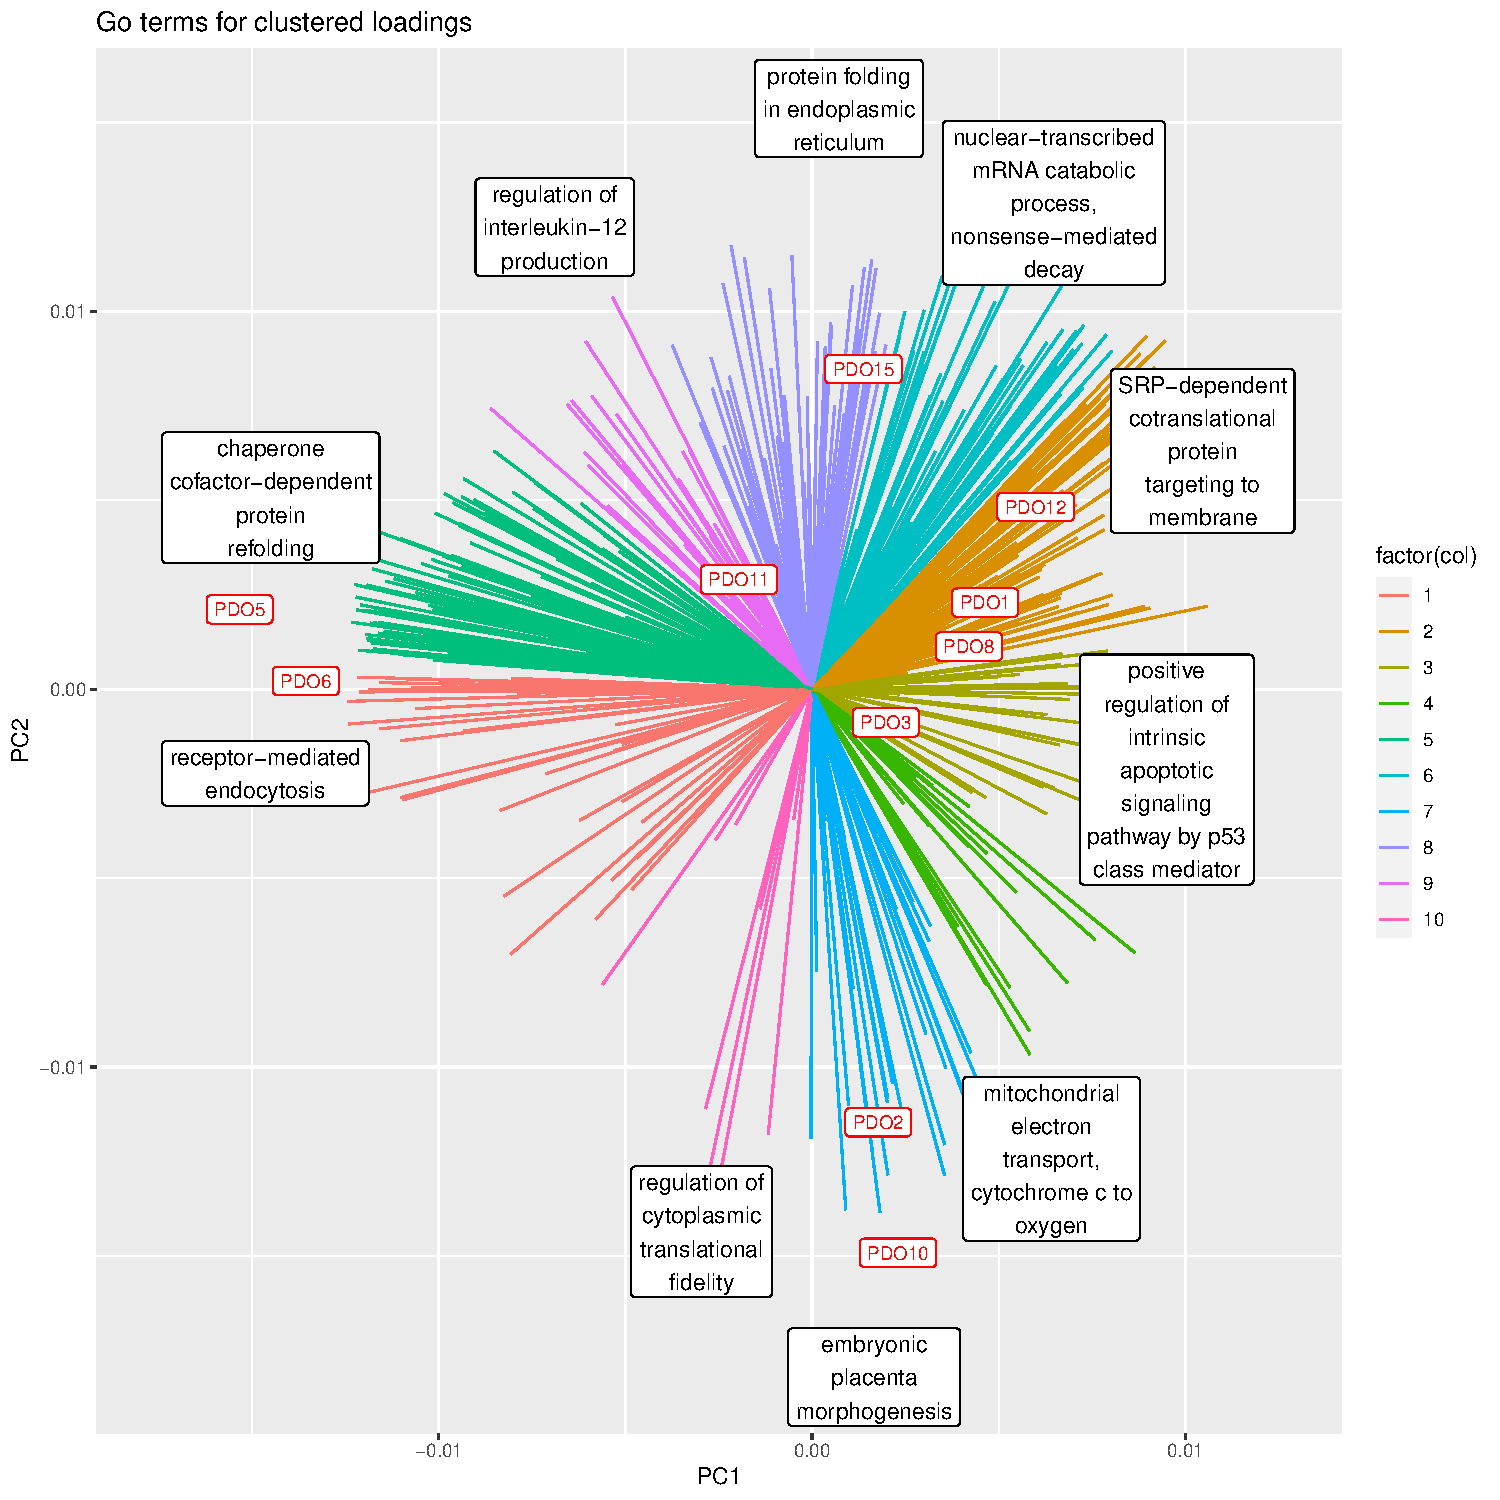
\includegraphics[width=5.2in]{/Users/morril01/Documents/PhD/other_repos/Vias_Brenton/RNASeq_DE_resistant_sensitive/figures/PCA_RNASeq/grouped_loadings_GO_subset.pdf}
\caption{Annotation of the loadings in the first two PCs\label{anno}}
\end{figure}

\clearpage
\subsection{Some general comments about the RNA-Seq}
\begin{itemize}
\item Although I am not 100\% satisfied with the conclusions yet, I think it is in general difficult to draw any conclusion from a PCA in which we have such few samples, and don't expect a clustering (e.g. from biological or technical replicates). Perhaps the cluster of PDO5 and
PDO6 on one hand, and of PDO2 and PDO10 on the other, is the best we can aspire to find 
\item Florian thought that the way forward with the transcriptomics was doing pathway enrichment analyses similar to those I have shown here
\item I will continue with the CN/GE correlation analysis with (1) the subset of organoids (2) considering TPM instead of DESeq2 counts
\end{itemize}


\end{document}